%% abtex2-modelo-relatorio-tecnico.tex, v-1.9.7 laurocesar
%% Copyright 2012-2018 by abnTeX2 group at http://www.abntex.net.br/ 
%%
%% This work may be distributed and/or modified under the
%% conditions of the LaTeX Project Public License, either version 1.3
%% of this license or (at your option) any later version.
%% The latest version of this license is in
%%   http://www.latex-project.org/lppl.txt
%% and version 1.3 or later is part of all distributions of LaTeX
%% version 2005/12/01 or later.
%%
%% This work has the LPPL maintenance status `maintained'.
%% 
%% The Current Maintainer of this work is the abnTeX2 team, led
%% by Lauro César Araujo. Further information are available on 
%% http://www.abntex.net.br/
%%
%% This work consists of the files abntex2-modelo-relatorio-tecnico.tex,
%% abntex2-modelo-include-comandos and abntex2-modelo-references.bib
%%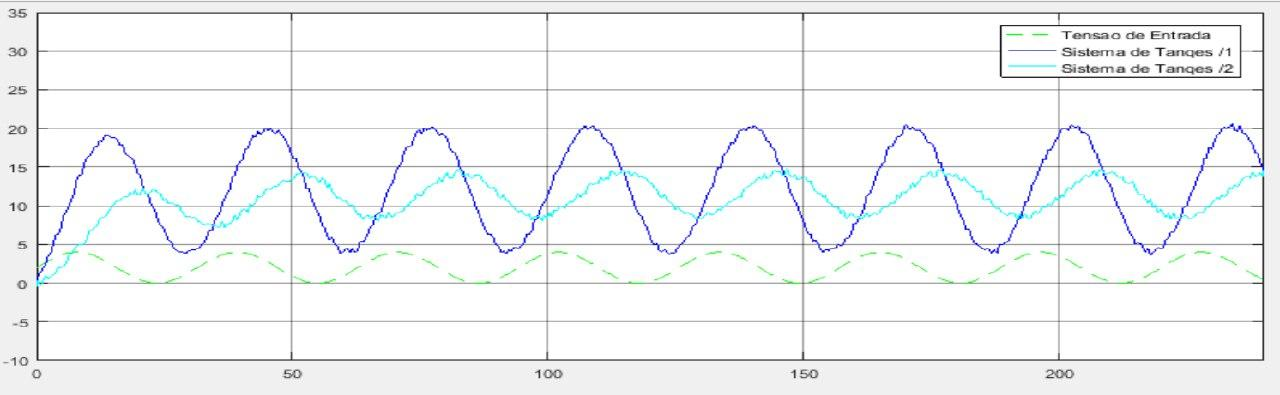
\includegraphics[scale=0.30]{./imagens/pt3/0.2rad.jpg}

% ------------------------------------------------------------------------
% ------------------------------------------------------------------------
% abnTeX2: Modelo de Relatório Técnico/Acadêmico em conformidade com 
% ABNT NBR 10719:2015 Informação e documentação - Relatório técnico e/ou
% científico - Apresentação
% ------------------------------------------------------------------------ 
% ------------------------------------------------------------------------

\documentclass[
	% -- opções da classe memoir --
	12pt,				% tamanho da fonte
	openany,			% capítulos começam em pág ímpar (insere página vazia caso preciso)
	oneside,			% para impressão em recto e verso. Oposto a oneside
	a4paper,			% tamanho do papel. 
	% -- opções da classe abntex2 --
	%chapter=TITLE,		% títulos de capítulos convertidos em letras maiúsculas
	%section=TITLE,		% títulos de seções convertidos em letras maiúsculas
	%subsection=TITLE,	% títulos de subseções convertidos em letras maiúsculas
	%subsubsection=TITLE,% títulos de subsubseções convertidos em letras maiúsculas
	% -- opções do pacote babel --
	english,			% idioma adicional para hifenização
	french,				% idioma adicional para hifenização
	spanish,			% idioma adicional para hifenização
	brazil,				% o último idioma é o principal do documento
	]{abntex2}

%\documentclass[12pt,a4paper,openany,oneside]{abntex2}
% ---
% PACOTES
% ---

% ---
% Pacotes fundamentais 
% ---
\usepackage{lmodern}			% Usa a fonte Latin Modern
\usepackage[T1]{fontenc}		% Selecao de codigos de fonte.
\usepackage[utf8]{inputenc}		% Codificacao do documento (conversão automática dos acentos)
\usepackage{indentfirst}		% Indenta o primeiro parágrafo de cada seção.
\usepackage{color}				% Controle das cores
\usepackage{graphicx}			% Inclusão de gráficos
\usepackage{microtype} 			% para melhorias de justificação
\usepackage{nameref}
\usepackage{chngcntr}
\counterwithin{equation}{chapter}
\counterwithin{figure}{chapter}
\counterwithin{table}{chapter}
% ---

% ---
% Pacotes adicionais, usados no anexo do modelo de folha de identificação
% ---
\usepackage{multicol}
\usepackage{multirow}
% ---
	
% ---
% Pacotes adicionais, usados apenas no âmbito do Modelo Canônico do abnteX2
% ---
\usepackage{lipsum}				% para geração de dummy text
% ---

% ---
% Pacotes de citações
% ---
\usepackage[brazilian,hyperpageref]{backref}	 % Paginas com as citações na bibl
\usepackage[alf]{abntex2cite}	% Citações padrão ABNT

% --- 
% CONFIGURAÇÕES DE PACOTES
% --- 

% ---
% Configurações do pacote backref
% Usado sem a opção hyperpageref de backref
\renewcommand{\backrefpagesname}{Citado na(s) página(s):~}
% Texto padrão antes do número das páginas
\renewcommand{\backref}{}
% Define os textos da citação
\renewcommand*{\backrefalt}[4]{
	\ifcase #1 %
		Nenhuma citação no texto.%
	\or
		Citado na página #2.%
	\else
		Citado #1 vezes nas páginas #2.%
	\fi}%
% ---

% ---
% Informações de dados para CAPA e FOLHA DE ROSTO
% ---
\titulo{DCA0216.0 - SISTEMAS DE CONTROLE\\ Avaliação - Unidade 2}
\autor{
\vspace{0.8cm}
Kallil de A. Bezerra: 20180154987\\
\vspace{0.8cm}
}
\local{Brasil}
\data{Novembro de 2020}
\instituicao{%
  Universidade Federal do Rio Grande do Norte -- UFRN
  \par
  Departamento de Engenharia da Computação e Automação -- DCA}
\tipotrabalho{Relatório técnico}
% O preambulo deve conter o tipo do trabalho, o objetivo, 
% o nome da instituição e a área de concentração 
\preambulo{Modelo canônico de Relatório Técnico e/ou Científico em conformidade
com as normas ABNT apresentado à comunidade de usuários \LaTeX.}
% ---

% ---
% Configurações de aparência do PDF final

% alterando o aspecto da cor azul
\definecolor{blue}{RGB}{41,5,195}

% informações do PDF
\makeatletter
\hypersetup{
     	%pagebackref=true,
		pdftitle={\@title}, 
		pdfauthor={\@author},
    	pdfsubject={\imprimirpreambulo},
	    pdfcreator={LaTeX with abnTeX2},
		pdfkeywords={abnt}{latex}{abntex}{abntex2}{relatório técnico}, 
		colorlinks=true,       		% false: boxed links; true: colored links
    	linkcolor=blue,          	% color of internal links
    	citecolor=blue,        		% color of links to bibliography
    	filecolor=magenta,      		% color of file links
		urlcolor=blue,
		bookmarksdepth=4
}
\makeatother
% --- 

% --- 
% Espaçamentos entre linhas e parágrafos 
% --- 

% O tamanho do parágrafo é dado por:
\setlength{\parindent}{1.3cm}

% Controle do espaçamento entre um parágrafo e outro:
\setlength{\parskip}{0.2cm}  % tente também \onelineskip

% ---
% compila o indice
% ---
\makeindex
% ---

% ----
% Início do documento
% ----
\begin{document}

% Seleciona o idioma do documento (conforme pacotes do babel)
%\selectlanguage{english}
\selectlanguage{brazil}

% Retira espaço extra obsoleto entre as frases.
\frenchspacing 

% ----------------------------------------------------------
% ELEMENTOS PRÉ-TEXTUAIS
% ----------------------------------------------------------
% \pretextual

% ---
% Capa
% ---
\imprimircapa
% ---

% ---
% Folha de rosto
% (o * indica que haverá a ficha bibliográfica)
% ---
\imprimirfolhaderosto*
% ---

% ---
% Anverso da folha de rosto:
% ---

{
\ABNTEXchapterfont


% ---
% RESUMO
% ---

% resumo na língua vernácula (obrigatório)
\setlength{\absparsep}{18pt} % ajusta o espaçamento dos parágrafos do resumo
\begin{resumo}
 O controlador Proporcional-Integral-Derivativo (PID) é o mais usado na indústria e tem sido utilizado há bastante tempo no controle industrial. A adoção dele se dá pelo seu desempenho confiável mesmo em condições adversas, além disso também apresenta uma certa facilidade de implementação. 
 
 Ele é composto por três coeficientes, que podem ser alterados para se obter a resposta ideal. Neste relatório será elaborado um controlador para indústria química, apresentando \textit{overshoot} de 20\% e tempo de estabilização de 600 segundos, ou 10 minutos.

 \noindent
 \textbf{Palavras-chaves}: Sistema de Controle. PID. Sistemas Dinâmicos.
\end{resumo}
% ---

% ---
% inserir lista de ilustrações
% ---
\pdfbookmark[0]{\listfigurename}{lof}
\listoffigures*
\cleardoublepage
% ---

% ---
% inserir lista de tabelas
% ---
\pdfbookmark[0]{\listtablename}{lot}
\listoftables*
\cleardoublepage
% ---

% ---
% inserir lista de abreviaturas e siglas
% ---
%\begin{siglas}
%  \item[ABNT] Associação Brasileira de Normas Técnicas
%  \item[abnTeX] ABsurdas Normas para TeX
%\end{siglas}
% ---

% ---
% inserir lista de símbolos
% ---
%\begin{simbolos}
%  \item[$ \Gamma $] Letra grega Gama
%  \item[$ \Lambda $] Lambda
%  \item[$ \zeta $] Letra grega minúscula zeta
%  \item[$ \in $] Pertence
%\end{simbolos}
% ---

% ---
% inserir o sumario
% ---
\pdfbookmark[0]{\contentsname}{toc}
\tableofcontents*
\cleardoublepage
% ---


% ----------------------------------------------------------
% ELEMENTOS TEXTUAIS
% ----------------------------------------------------------
\textual

% ----------------------------------------------------------
% Introdução (exemplo de capítulo sem numeração, mas presente no Sumário)
% ----------------------------------------------------------
\chapter*[Introdução]{Introdução}
\addcontentsline{toc}{chapter}{Introdução}

O controle automático tem desempenhado um papel vital no avanço da engenharia e da ciência. Além da sua importância em sistemas de veículos espaciais, sistemas robóticos, e semelhantes, o controle automático tornou-se uma importante parte da fabricação moderna e dos processos industriais. É possível citar o controle numérico de ferramentas e máquinas nas indústrias de manufatura, no projeto de sistemas de piloto automático em operações aeroespaciais e no projeto de carros e caminhões na indústria automobilística. O controle também é essencial no controle de pressão, temperatura, umidade e viscosidade nos processos industriais \cite{ogata}.


% Ogata - cap 5 - Transient and Steady-State Response Analyses
% 234/978 - sistemas de primeira ordem

% ----------------------------------------------------------
% PARTE - preparação da pesquisa
% ----------------------------------------------------------
\chapter{Embasamento teórico}

Em reações exotérmicas irreversíveis, reagentes de modo adiabático levam a altas temperaturas, portanto, para que haja um controle dessa temperatura, o calor gerado deve ser removido por resfriamento. Assumiremos que os reagentes estão perfeitamente misturados, e apenas uma única ação exotérmica irreversível de primeira ordem ocorre. Portanto, a variável a ser controlada é a temperatura do reator, $T$, e a variável manipulada é a temperatura de resfriamento, $T_R$. O sistema em questão é não-linear e é definido pelas seguintes equações de estado:

\begin{equation}
	\dot{C_A} = C_A + D_a(1-C_A)exp\left(T/\left(\frac{(1+T)}{\gamma}\right)\right) - (C_f - 1)
\end{equation}

\begin{equation}
	\dot{T} = T + B \cdot D_a(1-C_A)exp\left(T/\left(\frac{(1+T)}{\gamma}\right)\right) - \beta(T_R - T)
\end{equation}

Aqui temos $C_A$, que é a concentração do produto no reator, dado em $\frac{gmol}{L}$, $T$ é a temperatura do reator, variável controlada, dada em $Kelvin$, $T_R$ é a temperatura do resfriamento, variável manipulada, dada em $Kelvin$ também, e $C_f$ é a concentração da alimentação do equipamento, dada em $\frac{gmol}{L}$. Valores típicos dessas variáveis são dados na tabela \ref{tab:tabela_constantes}:

\begin{table}[h]
	\centering
	\begin{tabular}{ccc}
		\multicolumn{1}{c}{} 
	Constante & Valor &  \\ \hline
	$\gamma$ & 20 &  \\
	$D_a$ & 0.072 &  \\
	B & 8 &  \\
	$\beta$ & 0.3 &  \\
	$C_f$ & 1 & 
	\end{tabular}
	\caption{Valores do controlador PI}
	\label{tab:tabela_constantes}
\end{table}

Para o ponto de equilíbrio, usando $T_R=0$, $T=4.705K$, $C_A = 0.76456 \ \frac{gmol}{L}$, o sistema corresponde ao seguinte modelo linearizado:

\begin{equation}
	G(s) = \frac{0.005001s + 0.0003501}{s^2+0.02668s+0.0004545}
\end{equation}



\chapter{Desenvolvimento}

\section{Projetando o controlador PI}

É pedido que seja projetado um controlador PID, ou PI, para o sistema proposto, aplicando-o ao modelo não-linear. Devem ser considerador como critérios para o projeto um sobressinal máximo de 20\% e um tempo de estabilização de 10 minutos, o controlador também deve ser discretizado para uma amostragem de 0.1 minutos, ou 6 segundos.

Podemos começar analisando o critério de \textit{overshoot} e tempo de estabilização, que será convertido em segundos. Serão usadas as seguintes fórmulas:

\begin{equation}
	\xi = \frac{\ln(overshoot)}{\sqrt{\pi^2+\ln^2overshoot}}
\end{equation}

E

\begin{equation}
	t_s(5\%) = \frac{3}{\xi\omega_n}
\end{equation}

Agora, aplicando as especificações de desempenho temos:

$$\xi = \frac{\ln(0,2)}{\sqrt{\pi^2 + \ln(0,2)}}$$

resultando em:

$$\xi = 0,45594$$

Agora, usando o requisito do tempo temos:

$$t_s(5\%) \leq 10 $$
$$10 = \frac{3}{\xi\omega_n}$$
$${\xi\omega_n} = 0,3$$

portanto, 

$$\omega_n = 0,65776$$

Agora, precisamos encontrar o $\omega_d$.

$$\omega_d = \omega \sqrt{1-\xi^2}$$
$$\omega_d = 0,5853$$

Assim, temos os polos de malha fechada, que são:

$$s_{1,2} = -0,3 \pm 05853i$$

Com os valores de $\omega_d$, $\omega$ e $\xi$ em mãos, podemos descobrir os ângulos, dessa forma obtemos: $\theta_1 = 178,8846 ^ {\circ}$ e $\theta_2 = 181,1153^{\circ}$. Também encontramos $\phi_1 = 0,1,1963^{\circ}$ e $\phi_2$ será calculado, para que o $z$ seja encontrado. Com o zero faltando encontrado, temos $z = 7,4693$. 

Com isso, construímos o seguinte controlador PI:

$$G_c(s) = \frac{(s+z)^2}{s}$$ 

$$G_c(s) = \frac{s^2 + 14,94s + 55,79}{s}$$

Então, temos $k_p = 14,93$ e $k_i = 55,79$.

Na discretização foi usado o método \textit{forward}, encontrando a seguinte forma:

$$G(z) = \frac{10z^2 - 5,07z + 0,649}{(z-1)}$$

Ao fim do relatório estão as anotações originais feitas para resolver a atividade proposta.

\newpage
\section{Simulação do controlador}

O projeto proposto deve ser simulado no Matlab, os gráficos serão apresentados a seguir, com o sinal de saída e controle, aplicando o degrau unitário. A simulação não conseguiu atender aos requisitos impostos, demorando $697$ segundos para acomodar, mas respeitou os $20\%$ de sobressinal.

\begin{figure}[h]
	\centering
	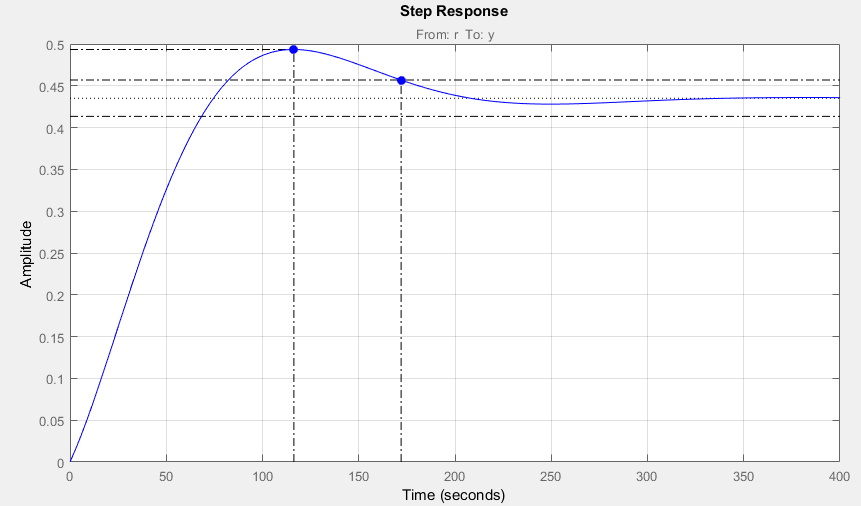
\includegraphics[scale=0.50]{imagens/2_matlab.PNG}
	\caption{Comportamento do sistema}
	\label{fig:sist_matlab}
\end{figure}

%\ref{fig:controladorPG10}


\clearpage

\postextual

% ----------------------------------------------------------
% Referências bibliográficas
% ----------------------------------------------------------
\bibliography{abntex2-modelo-references}

\phantompart

\printindex

\end{document}
